\input{../../headers/beamervideosHeadings}

\title{Fonctions de transfert dans le domaine de Laplace}

\setbeamertemplate{headline}[pagetitre]
\frame{\titlepage}

\usebackgroundtemplate%
{%
    \centering\includegraphics[width=\paperwidth]{../../headers/tableau}%
}

\setbeamertemplate{headline}[pagetitre]
\frame{
\frametitle{\inserttitle}

\begin{obj}
Déterminer la fonction de transfert qui régit le comportement d'un S.L.C.I.
\end{obj}

\begin{minipage}{0.46\linewidth}
\tableofcontents
\end{minipage}\hfill
\begin{minipage}{0.46\linewidth}
\begin{figure}[ht!]
\centering\includegraphics[width=0.5\linewidth]<2>{img/moteur}
\end{figure}
\end{minipage}
}

\section[Mise en équation]{Mise en équation (Moteur à Courant Continu $\frac{\omega_m}{u_m}$)}

\setbeamertemplate{headline}[renaud theme]
{\frame{
\frametitle{Mise en équation}

\begin{minipage}{0.47\linewidth}
\begin{eqnarray}
	\color<1>{blue}{u_m(t)=R_m\cdot i_m(t)+L_m\cdot \frac{d\ i_m(t)}{dt}+e(t)} \\
	\color<2>{blue}{e(t)=K_e\cdot \omega_m(t)} \\
	\color<2>{blue}{c_m(t)=K_i\cdot i_m(t)} \\
	\color<3>{blue}{J\cdot \frac{d\omega_m(t)}{dt}=c_m(t)}
\end{eqnarray}
\end{minipage}\hfill
\begin{minipage}{0.47\linewidth}
 \begin{overlayarea}{6.5cm}{4cm}
\only<1>{
 \begin{circuitikz}
\draw (0,3) to [R, l=$R$, i=$i_m$] (2.5,3);
\draw (2.5,3) to [L, l=$L$] (5,3);
\draw (5,0) to [V, v=$e(t)$] (5,3);
\draw (5,0) -- (0,0);
\draw[-triangle 45] (0,0.5) --  node[left] {$u_m(t)$} (0,2.5) ;
\end{circuitikz}}
\only<3>{ \centering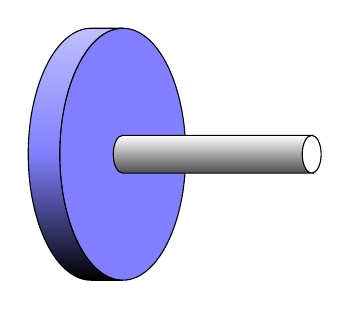
\begin{tikzpicture}[scale=0.8]
\draw[fill=blue!50](0,0) circle (1 and 2);
\draw[top color=blue!25,bottom color=black,middle color=blue!50] (-0.5,2) arc (90:270:1 and 2) -- ++(0.5,0) arc (-90:-270:1 and 2) -- cycle;
\draw[top color=white,bottom color=black!70] (0,3mm) arc (90:270:1.5mm and 3mm)--++(3cm,0) arc (-90:-270:1.5mm and 3mm)-- cycle;
\draw (3cm,3mm) arc (90:-90:1.5mm and 3mm);
\end{tikzpicture}}
\end{overlayarea}
\end{minipage}
}}

\setbeamertemplate{headline}[renaud theme]
{\frame{
\frametitle{Équation différentielle}
\begin{eqnarray}
\frac{u_m(t)}{K_e}=\frac{L_m\cdot J}{K_i\cdot K_e}\cdot\frac{d^2\omega_m(t)}{dt^2}+\frac{R_m\cdot J}{K_i\cdot K_e}\cdot\frac{d\omega_m(t)}{dt}+\omega_m(t)
\end{eqnarray}

Équation différentielle d'\textbf{ordre 2 avec second membre}. Méthode de résolution:
\begin{itemize}
 \item Recherche de la solution de l'équation sans second membre à l'aide du \textbf{discriminant},
 \item Recherche d'une \textbf{solution particulière} afin d'obtenir la solution générale.
\end{itemize}

Autre solution possible: \textbf{La transformée de Laplace} qui permet de résoudre des équations différentielles \textbf{linéaires} à \textbf{coefficients constants}.


}}

\section{Transformées de Laplace}

\setbeamertemplate{headline}[renaud theme]
{\frame{
\frametitle{Passage dans le domaine de Laplace}

\setcounter{equation}{0}

\begin{minipage}{0.47\linewidth}
\begin{eqnarray}
	u_m(t)=R_m\cdot i_m(t)+L_m\cdot \frac{d\ i_m(t)}{dt}+e(t) \\
	e(t)=K_e\cdot \omega_m(t) \\
	c_m(t)=K_i\cdot i_m(t) \\
	J\cdot \frac{d\omega_m(t)}{dt}=c_m(t)
\end{eqnarray}
\end{minipage}\hfill
\begin{minipage}{0.47\linewidth}
\only<2>{
Théorème de la dérivée première:\\ ~\ \\
	$L\left[\frac{df(t)}{dt}\right]=p\cdot F(p)-f(0^+)$
	Hypothèse:
	\begin{itemize}
	 \item Conditions initiales nulles (obligatoire pour la Fonction de Transfert)
	\end{itemize}
}
\only<3>{\begin{eqnarray}
	U_m(p)=R_m\cdot I_m(p)+L_m\cdot p\cdot I_m+E(p) \\
	E(p)=K_e\cdot \Omega_m(p) \\
	C_m(p)=K_i\cdot I_m(p) \\
	J\cdot p\cdot \Omega_m(p)=C_m(p)
\end{eqnarray}}
\end{minipage}
}}

\section{Fonction de transfert}

\setbeamertemplate{headline}[renaud theme]
{\frame{
\frametitle{Fonction de transfert}

\setcounter{equation}{4}

\only<1-3>{\begin{eqnarray}
	{\color<2->{vertf}{U_m(p)}}=R_m\cdot {\color<2->{red}{I_m(p)}}+L_m\cdot p\cdot {\color<2->{red}{I_m(p)}}+{\color<2->{red}{E(p)}} \\
	{\color<2->{red}{E(p)}}=K_e\cdot {\color<2->{vertf}{\Omega_m(p)}} \\
	{\color<2->{red}{C_m(p)}}=K_i\cdot {\color<2->{red}{I_m(p)}} \\
	J\cdot p\cdot {\color<2->{vertf}{\Omega_m(p)}}={\color<2->{red}{C_m(p)}}
\end{eqnarray}}
\only<3-6>{
\begin{eqnarray}
	\only<3>{{\color<2->{red}{I_m(p)}}=\frac{\color<2->{red}{C_m(p)}}{K_i} et\ {\color<2->{red}{E(p)}}=K_e\cdot {\color<2->{vertf}{\Omega_m(p)}} \Rightarrow} {\setcounter{equation}{9}\color<3->{vertf}{U_m(p)}}=R_m\cdot \frac{\color<2->{red}{C_m(p)}}{K_i}+L_m\cdot p\cdot \frac{\color<2->{red}{C_m(p)}}{K_i}+K_e\cdot {\color<2->{vertf}{\Omega_m(p)}}
\end{eqnarray}}
\only<5-7>{
\begin{eqnarray}
	\only<5>{{\color<2->{red}{C_m(p)}}=J\cdot p\cdot {\color<2->{vertf}{\Omega_m(p)}}\ (12) \Rightarrow} {\setcounter{equation}{10}\color<3->{vertf}{U_m(p)}}=R_m\cdot \frac{J\cdot p\cdot {\color<2->{vertf}{\Omega_m(p)}}}{K_i}+L_m\cdot p\cdot \frac{J\cdot p\cdot {\color<2->{vertf}{\Omega_m(p)}}}{K_i}+K_e\cdot {\color<2->{vertf}{\Omega_m(p)}}
\end{eqnarray}}
\only<6-8>{
\begin{eqnarray}
	{\setcounter{equation}{11}\color<3->{vertf}{U_m(p)}}=\left(\frac{R_m\cdot J\cdot p}{K_i}+\frac{L_m\cdot J\cdot p^2}{K_i}+K_e\right) \cdot {\color<2->{vertf}{\Omega_m(p)}}
\end{eqnarray}}
\only<8->{
\begin{eqnarray}
	\setcounter{equation}{12}\frac{\color<2->{vertf}{\Omega_m(p)}}{\color<3->{vertf}{U_m(p)}}=\frac{1}{K_e+\frac{R_m\cdot J}{K_i}\cdot p+\frac{L_m\cdot J}{K_i}\cdot p^2} 
\end{eqnarray}}
\only<9->{
Forme canonique:
\begin{eqnarray}
	\setcounter{equation}{13}\frac{\color<2->{vertf}{\Omega_m(p)}}{\color<3->{vertf}{U_m(p)}}=\frac{\frac{1}{K_e}}{
	 \tikzmark{b1} \only<9>{\myboxt{1}} \only<10->{\mybox{1}} +\frac{R_m\cdot J}{K_i\cdot K_e}\cdot p+\frac{L_m\cdot J}{K_i\cdot K_e}\cdot p^2} 
\end{eqnarray}}
\only<10->{\begin{tikzpicture}[overlay,remember picture]
    \draw[arrows=-latex] 
    ( $ (pic cs:b1) +(15pt,-4.5ex) $ ) -- 
    ( $ (pic cs:b1) +(8pt,-1ex) $ );
    \node[anchor=west]
    at ( $ (pic cs:b1) +(12pt,-6ex) $ )
    {Partie constante unitaire};
\end{tikzpicture}}


}}

\end{document}	

